% Provenance (never printed): see sources/outline_sources.md (Year 1: heat sources,
% radiogenic and secular cooling; heat-flow measurement; the steady conductive geotherm
% with heat production; convection against conduction; the lithosphere as a thermal
% boundary layer). Curves from figdata/bachelor-1/geotherms.py; exercise and problem
% values in the Book 3 scratch calculator calc/ch10.py.
\chapter{The Earth's Heat Budget}\label{ch:b1:heat-budget}

Under a mountain in the Japanese Alps, in an old mine cavity, a tank holding a
thousand tonnes of liquid scintillator watches for faint flashes of light. Most
come from antineutrinos made in the nuclear reactors of the country around it,
but some come from below: the uranium and thorium inside the Earth emit
antineutrinos as they decay, and these pass through the whole planet as if it
were empty. In 2135 days of counting the detector recorded 841 candidate
events, of which 106 were attributed to the Earth itself. From that handful of
flashes, its team estimated in 2011 that the decay of uranium and thorium heats
the Earth with about 20 terawatts. The planet as a whole loses about 47. This
chapter accounts for the difference: where the Earth's heat comes from, how
the heat flowing out of it is measured, how temperature rises with depth when
the heat is carried by conduction, why the \omterm{def:b1:layered-earth:layers}{mantle} must convect, and why the
plates are the cold upper boundary of that convection.

\begin{recall}
\omterm{def:b1:heat-budget:heat-flow}{Heat flows} from hot to cold; a rock's thermal conductivity $k$ measures how
easily heat crosses it, its thermal diffusivity $\kappa = k/(\rho c)$ how fast a
temperature change spreads (physics, University Year 2). Radioactive nuclei
decay with a fixed half-life (physics). The temperature rises with depth along
the \omterm{def:b1:heat-budget:geotherm}{geotherm}, and the \omterm{def:b1:layered-earth:layers}{mantle} convects (Book 2, grades 11 and 12). The
\omterm{def:b1:layered-earth:lithosphere}{lithosphere} is the strong outer shell of the Earth (\cref{ch:b1:layered-earth}).
\end{recall}

\section{Where the heat comes from}

\begin{definition}[Heat flow]\label{def:b1:heat-budget:heat-flow}
The \emph{heat flow}\index{heat flow} $q$ at a point of the Earth's surface, or
surface heat-flow density, is the power of internal origin that crosses the
surface there, per unit area, counted positive outwards. It is measured in
\unit{W.m^{-2}}, in practice in \unit{mW.m^{-2}}. Integrated over the whole
surface, it gives the Earth's heat loss $Q = \oint q\,\mathrm dS$.
\end{definition}

The \omterm{def:b1:heat-budget:heat-flow}{heat flow} has been measured at tens of thousands of sites. A compilation
of \num{38347} measurements, published in 2010, gives the mean values below,
with the oceans and the continents counted separately:
\begin{center}
\small
% ledger: dd10:split, dd10:total
\begin{tabular}{lccc}
\hline
 & area (\unit{m^2}) & heat loss (\unit{TW}) & mean \omterm{def:b1:heat-budget:heat-flow}{heat flow} (\unit{mW.m^{-2}}) \\
\hline
continents & \num{2.073e14} & 14.7 & 70.9 \\
oceans & \num{3.028e14} & 31.9 & 105.4 \\
whole Earth & \num{5.101e14} & 46.7 & 91.6 \\
\hline
\end{tabular}
\end{center}
The total, rounded to its uncertainty, is $Q = \qty[uncertainty-mode=separate]{47 \pm 2}{TW}$. Two thirds of
it leave through the ocean floor, which is younger and thinner than the
continents. It is a small flow: the Sun delivers about \qty{173000}{TW} to the
Earth, and the internal heat amounts to \qty{0.03}{\percent} of the energy
budget at the surface. % ledger: nasa:solar-mean
But it is the flow that drives volcanoes, plates and mountain building, and it
has two sources.

\begin{definition}[Radiogenic heat production]\label{def:b1:heat-budget:heat-production}
The \emph{radiogenic heat production}\index{radiogenic heat production} $A$ of
a rock is the heat released per unit volume and per unit time by the decay of
the radioactive nuclei it contains, in \unit{W.m^{-3}}, in practice in
\unit{\micro W.m^{-3}}. A rock of density $\rho$ containing mass fractions $C_i$
of the heat-producing elements, each releasing $H_i$ watts per kilogram of
element, has
\[
  A = \rho \sum_i C_i H_i .
\]
\end{definition}

Four isotopes produce almost all of this heat, because they are long-lived,
abundant enough and energetic: \ce{^{238}U}, \ce{^{235}U}, \ce{^{232}Th} and
\ce{^{40}K}. The heat per kilogram of each element is the heat per kilogram of
its radioactive isotope times that isotope's share of the element
(\cref{exo:b1:heat-budget:3}):
\begin{center}
\small
% ledger: dye:isotope-heat, iaea:isotopes
\begin{tabular}{lcccc}
\hline
isotope & half-life & heat per kg of isotope & share of the & heat per kg of element \\
 & (\unit{Gyr}) & (\unit{W.kg^{-1}}) & element (atoms) & (\unit{W.kg^{-1}}) \\
\hline
\ce{^{238}U} & 4.468 & \num{9.513e-5} & \qty{99.274}{\percent} & U: \num{9.85e-5} \\
\ce{^{235}U} & 0.704 & \num{5.685e-4} & \qty{0.720}{\percent} & \\
\ce{^{232}Th} & 14.0 & \num{2.628e-5} & almost all & Th: \num{2.63e-5} \\
\ce{^{40}K} & 1.248 & \num{2.847e-5} & \qty{0.0117}{\percent} & K: \num{3.40e-9} \\
\hline
\end{tabular}
\end{center}
Potassium releases thirty thousand times less heat per kilogram than uranium,
but it is a major element of many rocks, counted in per cent where uranium and
thorium are counted in parts per million. The rocks rich in all three are the
granites and their relatives; the poorest are the \omterm{def:b1:layered-earth:layers}{mantle} peridotites. A
compilation of \num{2188} analyses gives these medians, in \unit{\micro
W.m^{-3}}:
\begin{center}
\small
% ledger: vila:heat-production
\begin{tabular}{lclclc}
\hline
rhyolite & 2.55 & mudrocks & 1.44 & gabbro & 0.35 \\
granite & 2.43 & sandstones & 0.82 & basalt & 0.21 \\
granodiorite & 1.88 & carbonate rocks & 0.42 & ultramafic rocks & 0.11 \\
\hline
\end{tabular}
\end{center}
The spread within each group is wide: a quarter of granites produce less than
\qty{1.74}{\micro W.m^{-3}}, a quarter more than \qty{3.23}{\micro W.m^{-3}}.
The continental \omterm{def:b1:layered-earth:layers}{crust} is enriched in these elements, the oceanic \omterm{def:b1:layered-earth:layers}{crust} and the
\omterm{def:b1:layered-earth:layers}{mantle} depleted; but the \omterm{def:b1:layered-earth:layers}{mantle} is so large that it still holds a large share
of the planet's heat sources.

\begin{definition}[Secular cooling]\label{def:b1:heat-budget:secular-cooling}
\emph{Secular cooling}\index{secular cooling} is the part of the Earth's heat
loss supplied by the slow decrease of the temperature of its interior, \omterm{def:b1:layered-earth:layers}{mantle}
and core: the release of heat stored since the planet's formation, at a rate
$-\sum_j M_j c_j\,\mathrm dT_j/\mathrm dt$ for reservoirs of mass $M_j$,
specific heat $c_j$ and mean temperature $T_j$.
\end{definition}

Energy conservation gives the budget of the whole Earth: the heat lost at the
surface is the radiogenic production plus the \omterm{def:b1:heat-budget:secular-cooling}{secular cooling},
\[
  Q = H_{\text{rad}} + Q_{\text{sc}} .
\]
The geoneutrinos measure part of the first term: the 2011 result, which
combined two detectors, attributes \qty{20}{TW} to uranium and thorium, and
\ce{^{40}K}, whose antineutrinos are too weak to be detected that way, is
known to add about \qty{4}{TW}.
% ledger: kamland:2011
About half of the heat loss is therefore radiogenic, and the other half,
about \qty{23}{TW}, is \omterm{def:b1:heat-budget:secular-cooling}{secular cooling}. Part of that cooling is the core's: the
heat crossing the \omterm{def:b1:layered-earth:discontinuity}{core--mantle boundary} is estimated at \qtyrange{5}{15}{TW}.
These figures are uncertain: the measurement itself carries an uncertainty of
about \qty{9}{TW}, and the geoneutrino results so far only confine the
radiogenic part to \qtyrange{15}{41}{TW}, while Earth models of different
kinds spread from \qtyrange{14}{46}{TW}. The total, measured at the surface,
is the best-known term of the budget (figure below).
% ledger: dye:radiogenic

\begin{omfigure}
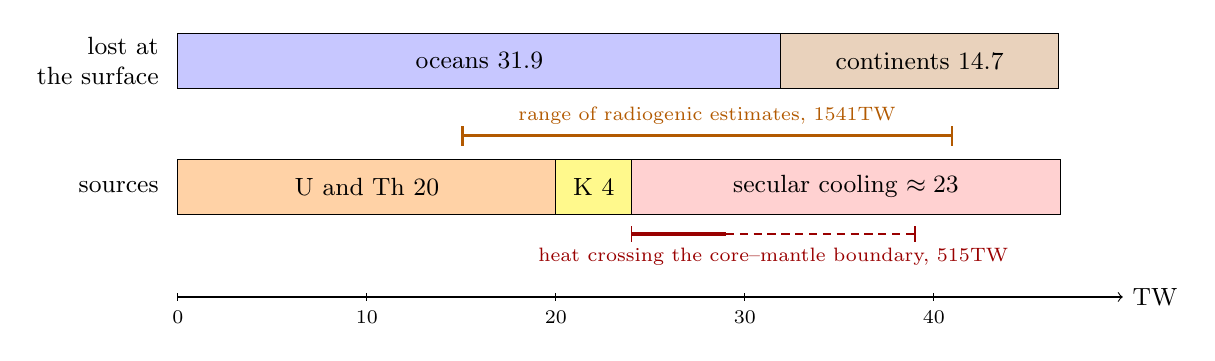
\begin{tikzpicture}[x=0.24cm, y=1cm, font=\small]
% ledger: dd10:split, kamland:2011, dye:radiogenic
% losses
\fill[blue!22] (0,1.6) rectangle (31.9,2.3);
\fill[brown!35] (31.9,1.6) rectangle (46.6,2.3);
\draw (0,1.6) rectangle (46.6,2.3);
\draw (31.9,1.6) -- (31.9,2.3);
\node at (15.95,1.95) {oceans 31.9};
\node at (39.25,1.95) {continents 14.7};
\node[anchor=east, align=right, font=\small] at (-0.5,1.95) {lost at\\the surface};
% sources
\fill[orange!35] (0,0) rectangle (20,0.7);
\fill[yellow!45] (20,0) rectangle (24,0.7);
\fill[red!18] (24,0) rectangle (46.7,0.7);
\draw (0,0) rectangle (46.7,0.7);
\draw (20,0) -- (20,0.7) (24,0) -- (24,0.7);
\node at (10,0.35) {U and Th 20};
\node at (22,0.35) {K 4};
\node at (35.35,0.35) {secular cooling $\approx 23$};
\node[anchor=east, align=right] at (-0.5,0.35) {sources};
% core part of secular cooling (range)
\draw[red!60!black, very thick] (24,-0.25) -- (29,-0.25);
\draw[red!60!black, thick, densely dashed] (29,-0.25) -- (39,-0.25);
\draw[red!60!black] (24,-0.15) -- (24,-0.35) (39,-0.15) -- (39,-0.35);
\node[anchor=north, font=\scriptsize, red!60!black] at (31.5,-0.3) {heat crossing the core--mantle boundary, \qtyrange{5}{15}{TW}};
% radiogenic range
\draw[|-|, orange!70!black, thick] (15,1.0) -- (41,1.0);
\node[anchor=south, font=\scriptsize, orange!70!black] at (28,1.02) {range of radiogenic estimates, \qtyrange{15}{41}{TW}};
% axis
\draw[->] (0,-1.05) -- (50,-1.05) node[right] {TW};
\foreach \x in {0,10,20,30,40} {\draw (\x,-1.0) -- (\x,-1.1) node[below, font=\scriptsize] {\x};}
\end{tikzpicture}

\par\smallskip{\small The Earth's heat budget. Top: the heat lost through the
ocean floor and the continents, \qty[uncertainty-mode=separate]{47 \pm 2}{TW} in all. Bottom: its sources,
with the radiogenic part of uranium and thorium measured by geoneutrinos and
that of potassium estimated; the rest, by difference, is \omterm{def:b1:heat-budget:secular-cooling}{secular cooling}, of
which the core supplies a poorly known part. The orange bar shows the range
of the radiogenic part allowed by the geoneutrino measurements.}
\label{fig:b1:heat-budget:budget}
\end{omfigure}

Radiogenic heat was larger in the past, because the isotopes were more
abundant: \ce{^{235}U} and \ce{^{40}K}, the short-lived ones, then contributed
much more (Book 2, grade 12). The Earth's heat engine is running down slowly,
on both counts.

\section{Measuring the heat flow}

\omterm{def:b1:heat-budget:heat-flow}{Heat flow} is not measured directly: it is computed from a temperature gradient
and a conductivity.

\begin{proposition}[Fourier's law]\label{prop:b1:heat-budget:fourier}
In a medium of thermal conductivity $k$, heat is conducted down the
temperature gradient at a rate per unit area proportional to it. With $z$ the
depth, counted positive downwards, and $q$ counted positive upwards,
\[
  q = k\,\frac{\mathrm dT}{\mathrm dz} .
\]
\end{proposition}
\admitted

The law is established in the physics books' University Year 2 volume. Most
rocks conduct heat at \qtyrange{1.5}{3}{W.m^{-1}.K^{-1}} below
\qty{200}{\celsius}, less when hot; models of continental \omterm{def:b1:heat-budget:heat-flow}{heat flow} give the
granitic upper \omterm{def:b1:layered-earth:layers}{crust} about \qty{2.7}{W.m^{-1}.K^{-1}};
% ledger: delaney:conductivity, roy:granitic-k
a gradient of \qty{25}{K.km^{-1}} in it means a \omterm{def:b1:heat-budget:heat-flow}{heat flow} of about
\qty{70}{mW.m^{-2}}.

When the rocks crossed by a borehole have different conductivities, the
gradient changes from one to the next, but the \omterm{def:b1:heat-budget:heat-flow}{heat flow} does not, as long as
no heat is produced or stored between them. The following proposition turns
that into a test.

\begin{proposition}[Bullard plot]\label{prop:b1:heat-budget:bullard}
Let $R(z) = \int_0^z \mathrm d\zeta/k(\zeta)$ be the thermal resistance, per
unit area, of the rocks between the surface and the depth $z$, in
\unit{m^2.K.W^{-1}}. If the \omterm{def:b1:heat-budget:heat-flow}{heat flow} $q$ is the same at every depth of a
borehole, the temperature is a linear function of the thermal resistance:
$T(z) = T_0 + q\,R(z)$.
\end{proposition}

\begin{proof}
By Fourier's law, $\mathrm dT/\mathrm dz = q/k(z)$. Integrating from $0$ to
$z$ with $q$ constant, $T(z) - T_0 = q\int_0^z \mathrm d\zeta/k(\zeta) = q\,R(z)$.
\end{proof}

\begin{method}[The heat flow from a borehole]\label{met:b1:heat-budget:borehole}
\begin{enumerate}
  \item Log the temperature down the borehole long after drilling, when the
        disturbance of the drilling fluid has died away, and set aside the
        shallowest tens of metres, which follow the seasons.
  \item Measure the conductivity of core samples of each rock crossed, in the
        laboratory, and compute the thermal resistance $R(z)$ at each logged
        depth.
  \item Plot $T$ against $R$: the slope of the straight line is the \omterm{def:b1:heat-budget:heat-flow}{heat flow}.
        A bend reveals water flowing through the rocks, a past change of
        surface temperature, or an error in a conductivity.
  \item Correct, where needed, for the relief, which bends the isotherms
        below hills and valleys, and for the slow warming since the last
        glaciation, which still disturbs the upper kilometre or so.
\end{enumerate}
\end{method}

At sea, a borehole is not needed. The temperature at the bottom of the deep
ocean is very steady, so that a few metres of soft sediment already carry the
equilibrium gradient. A steel lance carrying a row of temperature sensors is
dropped from a ship and driven into the sediment by a heavy weight
(figure below); the sensors record the gradient, and a
heat pulse sent along the lance gives the sediment's conductivity in place.
The ocean floor has one trap. On young \omterm{def:b1:layered-earth:layers}{crust}, sea water circulates through the
cracked basalt and carries much of the heat away by advection, so that the
measured conductive \omterm{def:b1:heat-budget:heat-flow}{heat flow} falls well short of the true loss. The loss
through the youngest ocean floor is therefore computed from the cooling model
of \cref{sec:b1:heat-budget:boundary-layer}, calibrated on old \omterm{def:b1:layered-earth:layers}{crust} where
circulation has stopped: this computed part, \qty{23.1}{TW}, is about half
the global total. % ledger: dd10:young-ocean

\begin{omfigure}
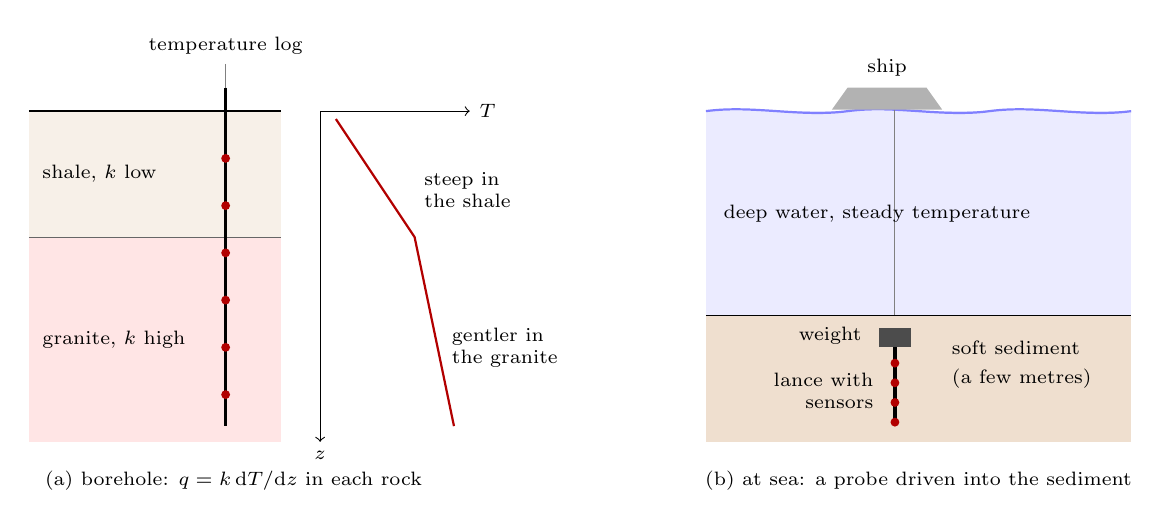
\begin{tikzpicture}[font=\scriptsize, x=1cm, y=1cm]
% --- left: borehole on land ---
\fill[brown!12] (0,0) rectangle (3.2,-1.6);
\fill[red!10] (0,-1.6) rectangle (3.2,-4.2);
\draw[thick] (0,0) -- (3.2,0);
\node[anchor=west] at (0.05,-0.8) {shale, $k$ low};
\node[anchor=west] at (0.05,-2.9) {granite, $k$ high};
\draw[black!60] (0,-1.6) -- (3.2,-1.6);
\draw[very thick] (2.5,0.3) -- (2.5,-4.0);
\draw[gray] (2.5,0.6) -- (2.5,0.3);
\foreach \y in {-0.6,-1.2,-1.8,-2.4,-3.0,-3.6} {\fill[red!70!black] (2.5,\y) circle (1.6pt);}
\node[anchor=south] at (2.5,0.6) {temperature log};
% inset T(z)
\draw[->] (3.7,0) -- (5.6,0) node[right] {$T$};
\draw[->] (3.7,0) -- (3.7,-4.2) node[below] {$z$};
\draw[thick, red!70!black] (3.9,-0.1) -- (4.9,-1.6) -- (5.4,-4.0);
\node[anchor=west, align=left] at (4.9,-1.0) {steep in\\the shale};
\node[anchor=west, align=left] at (5.25,-3.0) {gentler in\\the granite};
\node[anchor=north] at (2.6,-4.45) {(a) borehole: $q = k\,\mathrm dT/\mathrm dz$ in each rock};
% --- right: probe at sea ---
\begin{scope}[xshift=8.6cm]
\fill[blue!8] (0,0) rectangle (5.4,-2.6);
\draw[blue!50, thick] (0,0) .. controls (0.6,0.08) and (1.2,-0.08) .. (1.8,0)
  .. controls (2.4,0.08) and (3.0,-0.08) .. (3.6,0) .. controls (4.2,0.08) and (4.8,-0.08) .. (5.4,0);
\fill[gray!60] (1.6,0.02) -- (3.0,0.02) -- (2.8,0.3) -- (1.8,0.3) -- cycle;
\node[anchor=south] at (2.3,0.32) {ship};
\draw[gray] (2.4,0.02) -- (2.4,-2.75);
\fill[brown!25] (0,-2.6) rectangle (5.4,-4.2);
\draw (0,-2.6) -- (5.4,-2.6);
\node[anchor=west] at (3.0,-3.0) {soft sediment};
\node[anchor=west] at (3.0,-3.4) {(a few metres)};
\fill[black!70] (2.2,-2.75) rectangle (2.6,-3.0);
\draw[very thick] (2.4,-3.0) -- (2.4,-4.0);
\foreach \y in {-3.2,-3.45,-3.7,-3.95} {\fill[red!70!black] (2.4,\y) circle (1.6pt);}
\node[anchor=east, align=right] at (2.1,-2.85) {weight};
\node[anchor=east, align=right] at (2.25,-3.55) {lance with\\sensors};
\node[anchor=west] at (0.1,-1.3) {deep water, steady temperature};
\node[anchor=north] at (2.7,-4.45) {(b) at sea: a probe driven into the sediment};
\end{scope}
\end{tikzpicture}

\par\smallskip{\small Measuring the \omterm{def:b1:heat-budget:heat-flow}{heat flow} (schematic, not to scale). (a) On
land, the temperature is logged down a borehole once it has returned to
equilibrium, and the conductivity of each rock is measured on cores: the
gradient is steeper where the conductivity is lower, and the \omterm{def:b1:heat-budget:heat-flow}{heat flow}, their
product, is the same. (b) At sea, a lance with sensors is driven a few metres
into the sediment of the ocean floor.}
\label{fig:b1:heat-budget:measure}
\end{omfigure}

\begin{inthefield}[Heat flow at sea]
\begin{minipage}[t]{0.55\linewidth}\vspace{0pt}
On a research ship, the heat-flow probe is a heavy lance hung from the stern
crane. It is lowered on the ship's cable to just above the sea floor, then let
go: the weight drives it into the sediment, and the crew waits on deck while
the sensors settle to the temperature of the mud, then pulls it out and moves
on to the next station a short way off. A line of such stations across a
ridge flank gives the decline of \omterm{def:b1:heat-budget:heat-flow}{heat flow} with the age of the floor, and the
scatter between neighbouring stations shows where water is flowing through the
\omterm{def:b1:layered-earth:layers}{crust} below.
\end{minipage}\hfill
\begin{minipage}[t]{0.42\linewidth}\vspace{0pt}
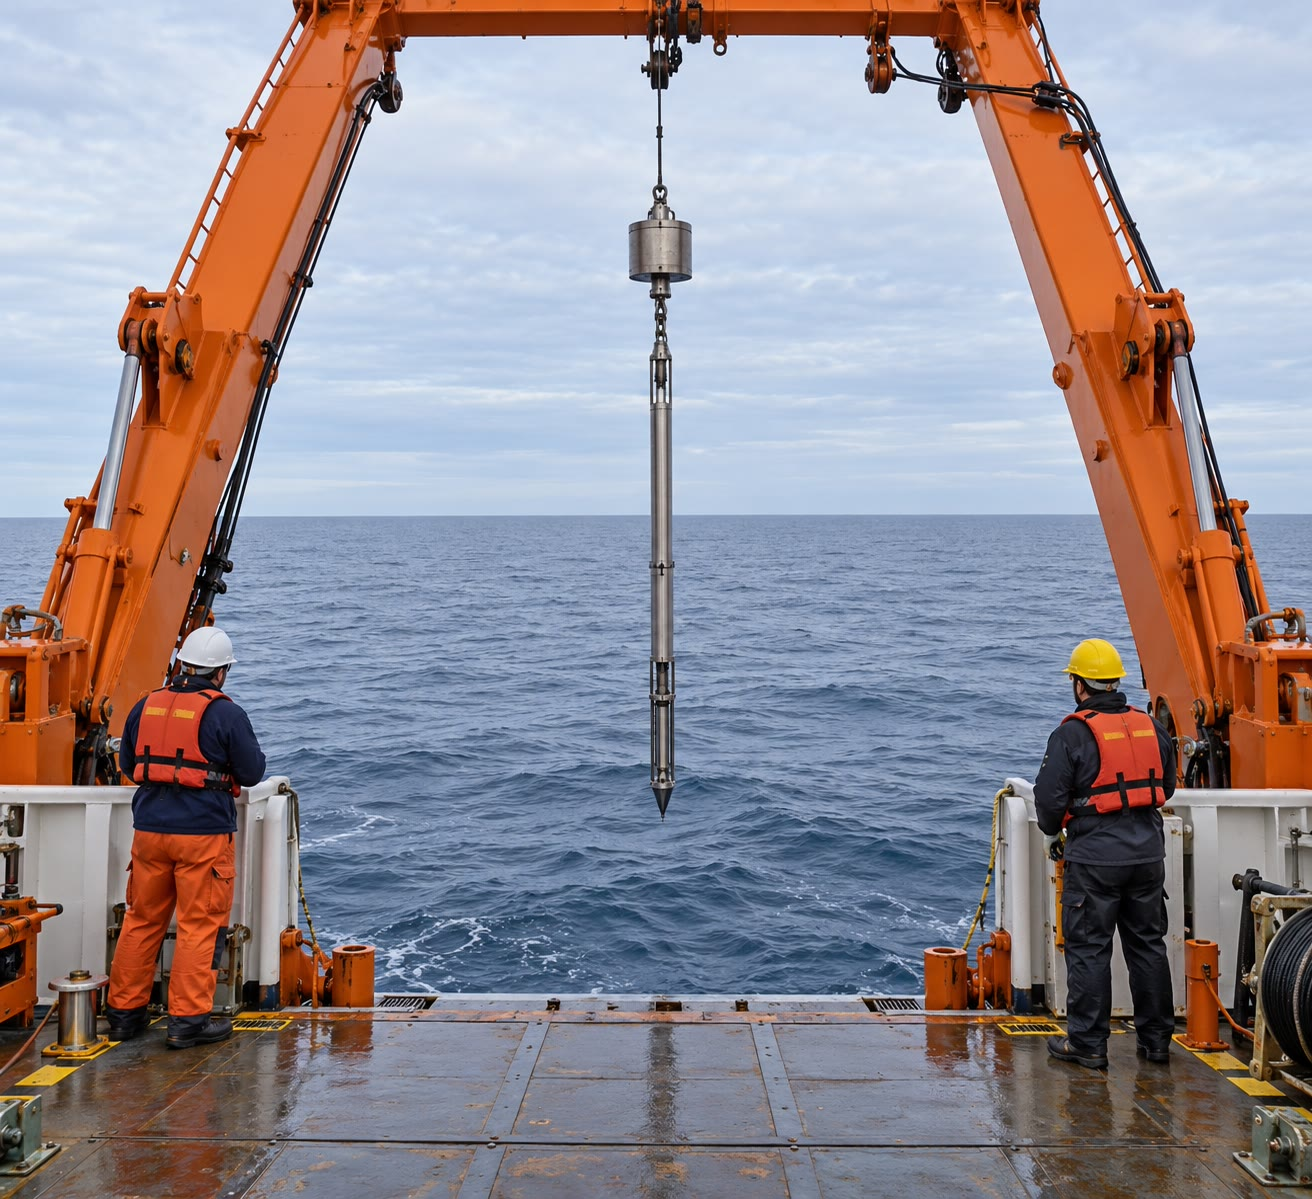
\includegraphics[width=\linewidth]{images/book3/ai/b1-heatflow-probe.jpg}

{\scriptsize A heat-flow probe hanging from the stern crane of a research ship
(AI-generated illustration).}
\end{minipage}
\end{inthefield}

\section{The steady conductive geotherm}

\begin{definition}[Geotherm]\label{def:b1:heat-budget:geotherm}
The \emph{geotherm}\index{geotherm} beneath a point of the surface is the
temperature as a function of depth there, $T(z)$. It is a steady
conductive geotherm when it does not change
with time and heat is carried along it by conduction alone.
\end{definition}

Within the \omterm{def:b1:layered-earth:lithosphere}{lithosphere}, far from active volcanoes and from water circulation,
the heat is carried by conduction, and on a scale of millions of years the
\omterm{def:b1:heat-budget:geotherm}{geotherm} is steady. Its shape then follows from an energy balance.

\begin{theorem}[Steady conduction with heat production]\label{thm:b1:heat-budget:balance}
Along a steady conductive \omterm{def:b1:heat-budget:geotherm}{geotherm}, in a medium of uniform conductivity $k$ with
heat production $A(z)$ and no horizontal flow of heat,
\[
  \frac{\mathrm dq}{\mathrm dz} = -A(z), \qquad\text{that is}\qquad
  k\,\frac{\mathrm d^2T}{\mathrm dz^2} = -A(z).
\]
\end{theorem}

\begin{proof}
Consider a horizontal slab of area $S$ between the depths $z$ and $z +
\mathrm dz$. Heat enters through its base at the rate $q(z + \mathrm dz)\,S$,
leaves through its top at the rate $q(z)\,S$, and is produced inside at the
rate $A(z)\,S\,\mathrm dz$. In a steady state no heat is stored, so
$q(z)\,S = q(z + \mathrm dz)\,S + A(z)\,S\,\mathrm dz$, which gives
$\mathrm dq/\mathrm dz = -A$. By Fourier's law $q = k\,\mathrm dT/\mathrm dz$,
and with $k$ uniform, $k\,T'' = -A$.
\end{proof}

Read from the surface down, the \omterm{def:b1:heat-budget:heat-flow}{heat flow} decreases with depth by the heat
produced above each level: what crosses the surface is the heat coming from
below plus all the heat produced on the way. Two distributions of $A$ give
closed forms.

\begin{proposition}[A uniform radiogenic layer]\label{prop:b1:heat-budget:uniform}
Let the heat production be $A$ from the surface down to the depth $h$ and zero
below, the surface be at temperature $T_0$, and the surface \omterm{def:b1:heat-budget:heat-flow}{heat flow} be $q_0$.
Then for $0 \le z \le h$
\[
  q(z) = q_0 - A z, \qquad T(z) = T_0 + \frac{q_0 z}{k} - \frac{A z^2}{2k},
\]
and below $h$ the \omterm{def:b1:heat-budget:heat-flow}{heat flow} is uniform, $q_m = q_0 - A h$, and the \omterm{def:b1:heat-budget:geotherm}{geotherm} a
straight line of slope $q_m/k$.
\end{proposition}

\begin{proof}
Integrate $\mathrm dq/\mathrm dz = -A$ from $0$ with $q(0) = q_0$: $q = q_0 -
Az$. Then $\mathrm dT/\mathrm dz = (q_0 - Az)/k$; integrating with $T(0) = T_0$
gives the parabola. Below $h$, $\mathrm dq/\mathrm dz = 0$ and $q$ keeps its
value at $h$.
\end{proof}

\begin{theorem}[Exponential heat production and the linear heat-flow relation]
\label{thm:b1:heat-budget:exponential}
Let the heat production decrease with depth as $A(z) = A_0 e^{-z/D}$, the \omterm{def:b1:heat-budget:heat-flow}{heat
flow} tend to $q_m$ at great depth, and the surface be at $T_0$. Then
\[
  q(z) = q_m + A_0 D\,e^{-z/D}, \qquad
  T(z) = T_0 + \frac{q_m z}{k} + \frac{A_0 D^2}{k}\bigl(1 - e^{-z/D}\bigr),
\]
and the surface \omterm{def:b1:heat-budget:heat-flow}{heat flow} is
\[
  q_0 = q_m + A_0 D .
\]
\end{theorem}

\begin{proof}
From \cref{thm:b1:heat-budget:balance}, $\mathrm dq/\mathrm dz =
-A_0e^{-z/D}$, so $q(z) = A_0 D e^{-z/D} + C$; as $z \to \infty$, $q \to C$,
hence $C = q_m$. At $z = 0$, $q_0 = q_m + A_0 D$. Then $\mathrm dT/\mathrm dz =
q/k = q_m/k + (A_0D/k)\,e^{-z/D}$, and integrating from $0$ with $T(0) = T_0$,
$T = T_0 + q_m z/k + (A_0 D^2/k)(1 - e^{-z/D})$.
\end{proof}

The last line is a prediction that can be tested at the surface. Granite
plutons in one region share the same deep \omterm{def:b1:heat-budget:heat-flow}{heat flow} $q_m$ and, if they differ
only by how rich they are in uranium, thorium and potassium, the same scale
$D$; then the \omterm{def:b1:heat-budget:heat-flow}{heat flow} measured over each pluton should be a linear function
of the heat production measured on its rocks, with slope $D$, a length, and
intercept $q_m$, the reduced \omterm{def:b1:heat-budget:heat-flow}{heat flow}, coming from below the radiogenic
layer. Francis Birch first observed such a line, reported in 1968, and the
same year three provinces were defined by their lines:
\begin{center}
\small
% ledger: roy:provinces, roy:linear-relation
\begin{tabular}{lcc}
\hline
province & intercept $q_m$ (\unit{mW.m^{-2}}) & slope $D$ (\unit{km}) \\
\hline
eastern United States & 33 & 7.5 \\
Basin and Range & 59 & 9.4 \\
Sierra Nevada & 17 & 10 \\
\hline
\end{tabular}
\end{center}
The intercepts, published as 0.8, 1.4 and $0.4\times\qty{e-6}{cal.cm^{-2}.s^{-1}}$,
are converted with $\qty{1}{\micro cal.cm^{-2}.s^{-1}} = \qty{41.84}{mW.m^{-2}}$
(\cref{exo:b1:heat-budget:4}). The slopes vary little, from 7 to \qty{10}{km}; the reduced \omterm{def:b1:heat-budget:heat-flow}{heat
flow} varies a lot, and maps of it show where the \omterm{def:b1:layered-earth:layers}{mantle} below is hot, as under
the stretched \omterm{def:b1:layered-earth:layers}{crust} of the Basin and Range. The uniform layer of
\cref{prop:b1:heat-budget:uniform} also gives a straight line, of slope $h$:
both models fit the data, but only the exponential one stays a straight line
of the same slope when the plutons are eroded to different depths
(\cref{exo:b1:heat-budget:10}), which is why it is preferred.

\begin{omfigure}
\begin{tikzpicture}
\begin{axis}[omdepth, width=0.82\linewidth, height=8.6cm, xmin=0, xmax=1800, ymin=0, ymax=250, axis x line=top, axis y line=left, axis line style={-}, clip=true,
  xlabel={temperature (\unit{\degreeCelsius})}, ylabel={depth (km)},
  tick label style={font=\scriptsize}, label style={font=\small},
  legend style={font=\scriptsize, at={(0.02,0.02)}, anchor=south west, draw=none, fill=white, fill opacity=0.85, text opacity=1},
  legend cell align=left]
\addplot[very thick, black!45] table[x=T, y=depth] {figdata/out/bachelor-1-geotherms-adiabat.dat};
\addlegendentry{mantle adiabat}
\addplot[very thick, red!75!black] table[x=T45, y=depth] {figdata/out/bachelor-1-geotherms-continental.dat};
\addlegendentry{$q_0 = \qty{70}{mW.m^{-2}}$}
\addplot[very thick, orange!80!black] table[x=T30, y=depth] {figdata/out/bachelor-1-geotherms-continental.dat};
\addlegendentry{$q_0 = \qty{55}{mW.m^{-2}}$}
\addplot[very thick, green!45!black] table[x=T15, y=depth] {figdata/out/bachelor-1-geotherms-continental.dat};
\addlegendentry{$q_0 = \qty{40}{mW.m^{-2}}$}
\addplot[thick, blue!70!black, densely dashdotted] table[x=T, y=depth] {figdata/out/bachelor-1-geotherms-oceanic.dat};
\addlegendentry{ocean floor \qty{60}{Myr} old}
\addplot[thin, dashed, red!75!black, forget plot] table[x=Tc45, y=depth] {figdata/out/bachelor-1-geotherms-continental.dat};
\addplot[thin, dashed, orange!80!black, forget plot] table[x=Tc30, y=depth] {figdata/out/bachelor-1-geotherms-continental.dat};
\addplot[thin, dashed, green!45!black, forget plot] table[x=Tc15, y=depth] {figdata/out/bachelor-1-geotherms-continental.dat};
\draw[densely dotted, black!60] (axis cs:0,35) -- (axis cs:1800,35);
\node[font=\scriptsize, anchor=south east] at (axis cs:1790,35) {Moho, \qty{35}{km}};
\fill (axis cs:1384.0,70.8) circle (1.6pt);
\fill (axis cs:1403.2,107.8) circle (1.6pt);
\fill (axis cs:1459.7,224.9) circle (1.6pt);
\node[font=\scriptsize, anchor=west] at (axis cs:1420,66) {\qty{71}{km}};
\node[font=\scriptsize, anchor=west] at (axis cs:1440,104) {\qty{108}{km}};
\node[font=\scriptsize, anchor=west] at (axis cs:1495,222) {\qty{225}{km}};
\end{axis}
\end{tikzpicture}

\par\smallskip{\small Steady conductive \omterm{def:b1:heat-budget:geotherm}{geotherms} of a continent with heat
production $A_0 = \qty{2.5}{\micro W.m^{-3}}$ decreasing over $D = \qty{10}{km}$,
$k = \qty{2.5}{W.m^{-1}.K^{-1}}$, for three surface \omterm{def:b1:heat-budget:heat-flow}{heat flows} (reduced \omterm{def:b1:heat-budget:heat-flow}{heat flow}
15, 30 and \qty{45}{mW.m^{-2}}). Each follows its conductive curve (dashed beyond)
down to the \omterm{def:b1:heat-budget:adiabat}{mantle adiabat}, which it meets at the dot: the base of the \omterm{def:b1:heat-budget:boundary-layer}{thermal
lithosphere}. The ocean-floor \omterm{def:b1:heat-budget:geotherm}{geotherm} is that of a half-space cooled for
\qty{60}{Myr}. Uniform conductivity is a simplification.}
\label{fig:b1:heat-budget:geotherms}
\end{omfigure}

\begin{method}[The temperature at depth beneath a pluton]\label{met:b1:heat-budget:moho}
\begin{enumerate}
  \item Measure the surface \omterm{def:b1:heat-budget:heat-flow}{heat flow} $q_0$ over the pluton (borehole method)
        and its heat production $A_0$ from its U, Th and K contents.
  \item From the line of the province, or with a value of $D$ of about
        \qty{10}{km}, compute $q_m = q_0 - A_0 D$.
  \item Apply \cref{thm:b1:heat-budget:exponential}. Below a few times $D$,
        $e^{-z/D}$ is negligible and the \omterm{def:b1:heat-budget:geotherm}{geotherm} is the straight line
        $T_0 + A_0D^2/k + q_m z/k$: the radiogenic layer has raised every deep
        temperature by $A_0D^2/k$.
\end{enumerate}
\end{method}

In the figure, the temperature at the \omterm{def:b1:layered-earth:discontinuity}{Moho} ranges from about \qty{320}{\degreeCelsius}
for the lowest \omterm{def:b1:heat-budget:heat-flow}{heat flow} to more than \qty{700}{\degreeCelsius} for the highest: the \omterm{def:b1:heat-budget:heat-flow}{heat flow} at the surface carries a direct reading of the
temperature of the deep \omterm{def:b1:layered-earth:layers}{crust}, which governs its strength
(\cref{ch:b1:stress-strain-rheology}).

\section{Conduction against convection}

Conduction is slow. How slow follows from the heat equation, which the physics
books derive from Fourier's law and the balance of
\cref{thm:b1:heat-budget:balance} with storage added: in one dimension, without
heat production,
$\partial T/\partial t = \kappa\,\partial^2 T/\partial z^2$.

\begin{proposition}[The conductive time scale]\label{prop:b1:heat-budget:timescale}
A temperature change imposed at a boundary of a conducting body spreads over a
distance $L$ in a time of order
\[
  \tau = \frac{L^2}{\kappa} .
\]
\end{proposition}

\begin{proof}
Write $z = L z^*$, $t = \tau t^*$, with $z^*$ and $t^*$ dimensionless. The heat
equation becomes $\partial T/\partial t^* = (\kappa\tau/L^2)\,\partial^2
T/\partial z^{*2}$. Its solutions vary on the scale $z^* \sim 1$ when $t^* \sim 1$
only if the coefficient is of order one, that is if $\tau \sim L^2/\kappa$.
\end{proof}

Rocks have $\kappa \approx \qty{e-6}{m^2.s^{-1}}$. The daily temperature cycle
reaches a few tens of centimetres into the ground, the yearly one a few metres, and
the warming since the last glaciation a kilometre or so. Across a \omterm{def:b1:layered-earth:lithosphere}{lithosphere}
\qty{100}{km} thick, $\tau = \qty{e16}{s}$, about \qty{300}{Myr}. Across the
\omterm{def:b1:layered-earth:layers}{mantle}, \qty{2900}{km} thick, $\tau = \qty{8.4e18}{s}$, or \qty{270}{Gyr}: sixty
times the age of the Earth, \qty{4.54}{Gyr}. % ledger: england:kelvin, usgs:age-earth
Conduction alone could not have brought the heat of the deep \omterm{def:b1:layered-earth:layers}{mantle} anywhere
near the surface. The \omterm{def:b1:layered-earth:layers}{mantle} convects, and in its interior the heat is carried
by the motion of the rock itself, at the speeds of the plates, centimetres per
year. % ledger: usgs:san-andreas

\begin{definition}[Mantle adiabat]\label{def:b1:heat-budget:adiabat}
The \emph{mantle adiabat}\index{mantle adiabat} is the \omterm{def:b1:heat-budget:geotherm}{geotherm} of the
well-mixed interior of the convecting \omterm{def:b1:layered-earth:layers}{mantle}: the temperature that \omterm{def:b1:layered-earth:layers}{mantle} rock
takes as it rises or sinks fast enough to exchange no heat with its
surroundings, cooling by expansion as it rises and warming by compression as it
sinks.
\end{definition}

Thermodynamics gives its gradient, $\mathrm dT/\mathrm dz = \alpha g T/c_p$,
with $\alpha$ the thermal expansivity and $c_p$ the specific heat (physics,
admitted here). It is small. A recent evaluation from mineral physics gives
\qty{0.54}{K.km^{-1}} at \qty{50}{km} depth, decreasing to \qty{0.36}{K.km^{-1}}
at \qty{410}{km}, then 0.41 to \qty{0.23}{K.km^{-1}} through the lower \omterm{def:b1:layered-earth:layers}{mantle},
with \qty{1646}{K} at \qty{50}{km} and \qty{2587}{K} at \qty{2800}{km}.
% ledger: katsura:adiabat
Extrapolated to the surface, the adiabat gives the \omterm{def:b1:layered-earth:layers}{mantle}'s potential
temperature, \qty{1619}{K} or about \qty{1350}{\degreeCelsius}: the temperature
the \omterm{def:b1:layered-earth:layers}{mantle} would have if it were brought up to the surface without exchanging
heat. The notion of potential temperature is defined, for the atmosphere and
the ocean, in \cref{ch:b1:fluid-envelopes-structure}. A temperature that
increases by only \qty{0.5}{K} per kilometre while the conductive \omterm{def:b1:heat-budget:geotherm}{geotherm} near
the surface climbs by \qty{25}{K} is the signature of convection.

\begin{history}[John Perry and the cooling Earth]
In 1862--1863 William Thomson, later Lord Kelvin, computed the age of the Earth
from its cooling. He treated it as a solid that had cooled by conduction from
a uniform temperature of about \qty{3900}{\degreeCelsius}; with the then mean
gradient he chose from the measurements of his time, about
\qty{36}{K.km^{-1}}, and a diffusivity of
\qty{1.2e-6}{m^2.s^{-1}}, the time needed to reach today's gradient was about
\qty{96}{Myr}, between bounds of 24 and \qty{400}{Myr} (\cref{exo:b1:heat-budget:9}). Geologists
found this far too short. In 1895, a year
before radioactivity was discovered, his former assistant John Perry pointed at
an assumption instead: if the interior were partly fluid and convected, it
would carry heat as if it had an enormous conductivity, and the whole interior,
not a thin outer shell, would feed the surface \omterm{def:b1:heat-budget:heat-flow}{heat flow}. His argument was
neglected and forgotten; \omterm{def:b1:layered-earth:layers}{mantle} convection, established long after, proved
him right: the deep \omterm{def:b1:layered-earth:layers}{mantle} cools by convection, and that is the \omterm{def:b1:heat-budget:secular-cooling}{secular
cooling} of the budget. % ledger: england:kelvin, england:perry
\end{history}

\begin{proposition}[Perry's well-stirred Earth]\label{prop:b1:heat-budget:perry}
Let a sphere of radius $R$ have a well-stirred interior at the uniform
temperature $T_i(t)$, with heat capacity $\rho c$ per unit volume, under a
conducting lid of thickness $L \ll R$ and conductivity $k$ whose surface is at
$\qty{0}{\degreeCelsius}$, and let there be no heat production. Then
\[
  T_i(t) = T_i(0)\,e^{-t/\tau_P}, \qquad \tau_P = \frac{RL}{3\kappa},
\]
and the surface \omterm{def:b1:heat-budget:heat-flow}{heat flow} $kT_i/L$ decays with the same time constant.
\end{proposition}

\begin{proof}
The lid being thin, it is in a steady state and carries the \omterm{def:b1:heat-budget:heat-flow}{heat flow}
$q = kT_i/L$. The interior loses its heat through the area $4\pi R^2$:
$\tfrac43\pi R^3\rho c\,\mathrm dT_i/\mathrm dt = -4\pi R^2 kT_i/L$, that is
$\mathrm dT_i/\mathrm dt = -3\kappa T_i/(RL)$ with $\kappa = k/(\rho c)$, whose
solution is the exponential with $\tau_P = RL/(3\kappa)$.
\end{proof}

For $R = \qty{6400}{km}$, $L = \qty{100}{km}$ and $\kappa =
\qty{e-6}{m^2.s^{-1}}$, $\tau_P = \qty{6.8}{Gyr}$: a convecting Earth keeps a
high \omterm{def:b1:heat-budget:heat-flow}{heat flow} for billions of years, where Kelvin's conducting Earth lost it
in tens of millions (\cref{exo:b1:heat-budget:11}).

\section{The lithosphere as a thermal boundary layer}\label{sec:b1:heat-budget:boundary-layer}

\begin{definition}[Thermal boundary layer, thermal lithosphere]\label{def:b1:heat-budget:boundary-layer}
In a convecting fluid, a \emph{thermal boundary layer}\index{thermal boundary
layer} is a layer along a boundary across which heat passes by conduction and
the temperature changes from that of the boundary to that of the well-mixed
interior. The \emph{thermal lithosphere}\index{thermal lithosphere} is the upper
thermal boundary layer of the \omterm{def:b1:layered-earth:layers}{mantle}: the outer shell of the Earth from the
surface down to the depth where the conductive \omterm{def:b1:heat-budget:geotherm}{geotherm} meets the \omterm{def:b1:heat-budget:adiabat}{mantle
adiabat}.
\end{definition}

The plates are the cold top of the \omterm{def:b1:layered-earth:layers}{mantle}'s convection, its upper boundary
layer. Their base, where the steep conductive \omterm{def:b1:heat-budget:geotherm}{geotherm} bends into the gentle
adiabat, lies at \qtyrange{70}{230}{km} in the figure of the \omterm{def:b1:heat-budget:geotherm}{geotherms}
for continental \omterm{def:b1:heat-budget:heat-flow}{heat flows} of 70 to \qty{40}{mW.m^{-2}}, in the range measured
by seismology (\cref{ch:b1:layered-earth}): the \omterm{def:b1:layered-earth:lithosphere}{lithosphere} defined by its
strength and the \omterm{def:b1:layered-earth:lithosphere}{lithosphere} defined by its temperature are roughly the same
shell, because strength depends on temperature. At the bottom of the \omterm{def:b1:layered-earth:layers}{mantle}, the
D$''$ layer is the lower boundary layer, heated from below by the core.

Under the oceans, the boundary layer is born at the ridge, where hot \omterm{def:b1:layered-earth:layers}{mantle}
rises to the surface, and thickens as the plate moves away and cools. The
cooling of a half-space from a uniform temperature, solved by Fourier and used
by Kelvin for the whole Earth, describes it well (\cref{ch:b1:rifts-ridges-margins}
and the Year 3 volume derive it): isotherms deepen as the square root of the
age of the floor (figure below), and the \omterm{def:b1:heat-budget:heat-flow}{heat flow}
decreases as
\[
  q(t) = \frac{C}{\sqrt t}, \qquad C \approx \qty{490}{mW.m^{-2}.Myr^{1/2}},
\]
the value used in the global budget. % ledger: dd10:young-ocean
At \qty{100}{Myr} the half-space has cooled to about \qty{130}{km} (\cref{exo:b1:heat-budget:12}). The real plate stops thickening sooner: seismic waves crossing the Pacific
are best fitted by a cooling plate that tends to a thickness of
\qtyrange{85}{95}{km}, the flattening of old sea floor met again in
\cref{ch:b1:rifts-ridges-margins}.
% ledger: fischer:lithosphere

The heat budget, the \omterm{def:b1:heat-budget:heat-flow}{heat flow} and the thermal structure of the plates come
together in the next chapters: the cooling plate subsides
(\cref{ch:b1:rifts-ridges-margins}), and the cold \omterm{def:b1:layered-earth:lithosphere}{lithosphere} sinking at
subduction zones is the downwelling of the convection it belongs to.

\begin{omfigure}
\begin{tikzpicture}
\begin{axis}[width=0.86\linewidth, height=5.6cm, xmin=0, xmax=100, ymin=0, ymax=170,
  y dir=reverse, axis x line=top, axis y line=left, axis line style={-}, clip=false,
  xlabel={age of the ocean floor (Myr), growing with distance from the ridge},
  ylabel={depth (km)}, tick label style={font=\scriptsize}, label style={font=\small}]
\addplot[fill=blue!12, draw=none] table[x=age, y=z1200] {figdata/out/bachelor-1-geotherms-isotherms.dat} \closedcycle;
\addplot[thick, blue!30!black] table[x=age, y=z400] {figdata/out/bachelor-1-geotherms-isotherms.dat};
\addplot[thick, blue!50!red] table[x=age, y=z800] {figdata/out/bachelor-1-geotherms-isotherms.dat};
\addplot[very thick, red!75!black] table[x=age, y=z1200] {figdata/out/bachelor-1-geotherms-isotherms.dat};
\node[font=\scriptsize, anchor=south, fill=blue!12, inner sep=1pt] at (axis cs:80,24) {\qty{400}{\degreeCelsius}};
\node[font=\scriptsize, anchor=south, fill=blue!12, inner sep=1pt] at (axis cs:80,55) {\qty{800}{\degreeCelsius}};
\node[font=\scriptsize, anchor=south, fill=blue!12, inner sep=1pt] at (axis cs:80,108) {\qty{1200}{\degreeCelsius}};
\node[font=\small] at (axis cs:60,72) {thermal lithosphere};
\node[font=\small] at (axis cs:55,150) {convecting mantle, about \qty{1350}{\degreeCelsius}};
\draw[->, thick, red!60!black] (axis cs:3,165) -- (axis cs:3,125);
\node[font=\scriptsize, anchor=west, red!60!black] at (axis cs:4,140) {rising under the ridge};
\draw[->, thick, black!60] (axis cs:30,5) -- (axis cs:70,5);
\node[font=\scriptsize, anchor=west] at (axis cs:70,5) {plate motion};
\end{axis}
\end{tikzpicture}

\par\smallskip{\small Isotherms in a cooling oceanic plate: a half-space
initially at \qty{1350}{\degreeCelsius}, cooled from its surface, with
$\kappa = \qty{e-6}{m^2.s^{-1}}$. Every isotherm deepens as the square root of
age; the shaded layer above the \qty{1200}{\degreeCelsius} isotherm is the \omterm{def:b1:heat-budget:boundary-layer}{thermal
lithosphere}. Arrows are schematic.}
\label{fig:b1:heat-budget:isotherms}
\end{omfigure}

\section{Exercises}

\begin{exercise}[$\star$]\label{exo:b1:heat-budget:1}
A borehole in granite of conductivity \qty{2.5}{W.m^{-1}.K^{-1}} shows a steady
gradient of \qty{22}{K.km^{-1}}. Compute the \omterm{def:b1:heat-budget:heat-flow}{heat flow}, and the power that
crosses one square kilometre of the surface there.
% ledger: delaney:conductivity
\end{exercise}

\begin{exercise}[$\star$]\label{exo:b1:heat-budget:2}
From the areas and mean \omterm{def:b1:heat-budget:heat-flow}{heat flows} of the continents (\qty{2.073e14}{m^2},
\qty{70.9}{mW.m^{-2}}) and the oceans (\qty{3.028e14}{m^2},
\qty{105.4}{mW.m^{-2}}), compute the heat loss of each, the total and the mean
\omterm{def:b1:heat-budget:heat-flow}{heat flow} over the Earth's surface (\qty{5.101e14}{m^2}). What fraction of the
\qty{173000}{TW} received from the Sun is it?
% ledger: dd10:split, nasa:solar-mean
\end{exercise}

\begin{exercise}[$\star$]\label{exo:b1:heat-budget:3}
From the table of the four isotopes, compute the heat released per kilogram of
natural uranium (\qty{99.274}{\percent} \ce{^{238}U} and \qty{0.720}{\percent}
\ce{^{235}U} of the atoms; their masses differ by about \qty{1}{\percent}, so
take these as mass fractions) and per kilogram of natural potassium, whose
\ce{^{40}K} makes \qty{0.0117}{\percent} of the atoms (take the mass of a
\ce{^{40}K} atom $39.96/39.10$ times the mean mass of a potassium atom).
% ledger: dye:isotope-heat, iaea:isotopes
\end{exercise}

\begin{exercise}[$\star$]\label{exo:b1:heat-budget:4}
Convert the intercepts of the three provinces, 0.8, 1.4 and
$0.4\times\qty{e-6}{cal.cm^{-2}.s^{-1}}$, into \unit{mW.m^{-2}}
($\qty{1}{cal} = \qty{4.184}{J}$). Predict the surface \omterm{def:b1:heat-budget:heat-flow}{heat flow} over a granite
of heat production \qty{3.0}{\micro W.m^{-3}} in each province.
% ledger: roy:provinces
\end{exercise}

\begin{exercise}[$\star\star$]\label{exo:b1:heat-budget:5}
A \omterm{def:b1:layered-earth:layers}{crust} has a uniform heat production of \qty{2.0}{\micro W.m^{-3}} in its upper
\qty{10}{km} and none below, a conductivity of \qty{2.5}{W.m^{-1}.K^{-1}}, a
surface \omterm{def:b1:heat-budget:heat-flow}{heat flow} of \qty{60}{mW.m^{-2}} and a surface temperature of
\qty{10}{\degreeCelsius}. Compute the temperature at \qty{10}{km}, the \omterm{def:b1:heat-budget:heat-flow}{heat flow}
below the radiogenic layer, and the temperature at the \omterm{def:b1:layered-earth:discontinuity}{Moho}, \qty{35}{km} down.
\end{exercise}

\begin{exercise}[$\star\star$]\label{exo:b1:heat-budget:6}
A borehole crosses \qty{300}{m} of shale ($k = \qty{1.5}{W.m^{-1}.K^{-1}}$), then
granite ($k = \qty{3.0}{W.m^{-1}.K^{-1}}$). The \omterm{def:b1:comparative-planetology:equilibrium-temperature}{equilibrium temperatures} are
\qty{12.0}{\degreeCelsius} at the surface, \qty{24.0}{\degreeCelsius} at
\qty{300}{m} and \qty{34.0}{\degreeCelsius} at \qty{800}{m}. Compute the
gradient and the \omterm{def:b1:heat-budget:heat-flow}{heat flow} in each rock, the thermal resistance at \qty{300}{m}
and at \qty{800}{m}, and the slope of the Bullard plot. Is the \omterm{def:b1:heat-budget:heat-flow}{heat flow}
constant?
\end{exercise}

\begin{exercise}[$\star\star$]\label{exo:b1:heat-budget:7}
With $\kappa = \qty{e-6}{m^2.s^{-1}}$, compute the conductive time scale for
$L = \qty{1}{m}$, \qty{10}{m}, \qty{100}{km} and \qty{2900}{km}, each in a
suitable unit. Which surface temperature cycles are still felt \qty{10}{m} below
the ground? Compare the last time with the age of the Earth.
% ledger: england:kelvin, usgs:age-earth
\end{exercise}

\begin{exercise}[$\star\star$]\label{exo:b1:heat-budget:8}
The \omterm{def:b1:heat-budget:adiabat}{mantle adiabat} is at \qty{1646}{K} at \qty{50}{km} depth, with a gradient of
\qty{0.54}{K.km^{-1}} there, decreasing to \qty{0.36}{K.km^{-1}} at \qty{410}{km}.
(a) Extrapolate it to the surface with the gradient at \qty{50}{km}, and give the
potential temperature in kelvins and in degrees Celsius. (b) Estimate the
temperature at \qty{410}{km} with the mean of the two gradients, and compare
with the published \qty{1799}{K} just above the discontinuity.
% ledger: katsura:adiabat
\end{exercise}

\begin{exercise}[$\star\star$]\label{exo:b1:heat-budget:9}
A half-space cooled from the uniform temperature $T_0$, its surface held at
$\qty{0}{\degreeCelsius}$, has after a time $t$ the surface gradient $G =
T_0/\sqrt{\pi\kappa t}$ (admitted). (a) Express $t$ in terms of $G$. (b) With
Kelvin's values, $T_0 = \qty{3900}{\degreeCelsius}$, $\kappa =
\qty{1.2e-6}{m^2.s^{-1}}$ and $G = 1/50$ of a degree Fahrenheit per foot,
compute $G$ in \unit{K.km^{-1}} and the age. (c) Redo it with $T_0 =
\qty{1300}{\degreeCelsius}$, $\kappa = \qty{e-6}{m^2.s^{-1}}$ and $G =
\qty{36}{K.km^{-1}}$.
% ledger: england:kelvin
\end{exercise}

\begin{exercise}[$\star\star\star$]\label{exo:b1:heat-budget:10}
A province is eroded: a thickness $e$ is removed from the top of every pluton,
the deep \omterm{def:b1:heat-budget:heat-flow}{heat flow} $q_m$ being unchanged. (a) In the exponential model, show
that the new surface heat production and \omterm{def:b1:heat-budget:heat-flow}{heat flow}, $A_0'$ and $q_0'$, still
satisfy $q_0' = q_m + A_0'D$. (b) In the uniform-layer model of thickness $h$,
show that a pluton eroded by $e$ lies on a line of slope $h - e$. (c) Plutons of
one province were eroded by different amounts. Which model predicts that they
still fall on a single line?
\end{exercise}

\begin{exercise}[$\star\star\star$]\label{exo:b1:heat-budget:11}
In Perry's model (\cref{prop:b1:heat-budget:perry}) take $R = \qty{6400}{km}$,
$\kappa = \qty{e-6}{m^2.s^{-1}}$, $k = \qty{3}{W.m^{-1}.K^{-1}}$ and an initial
interior temperature of \qty{1300}{\degreeCelsius}. (a) Compute $\tau_P$ for
lids of 50 and \qty{100}{km}. (b) For the \qty{50}{km} lid, compute the surface
\omterm{def:b1:heat-budget:heat-flow}{heat flow} at the start and after \qty{2}{Gyr}. (c) Kelvin's conducting
half-space with the same $k$ and $T_0$ has a surface \omterm{def:b1:heat-budget:heat-flow}{heat flow}
$kT_0/\sqrt{\pi\kappa t}$: compute it after \qty{2}{Gyr}, and compare.
% ledger: england:kelvin, england:perry
\end{exercise}

\begin{exercise}[$\star\star\star$]\label{exo:b1:heat-budget:12}
The surface \omterm{def:b1:heat-budget:heat-flow}{heat flow} of a cooling half-space is $q = k\,\Delta T/\sqrt{\pi\kappa t}$
(\cref{exo:b1:heat-budget:9}). (a) With $k = \qty{3}{W.m^{-1}.K^{-1}}$, $\kappa =
\qty{e-6}{m^2.s^{-1}}$ and $\Delta T = \qty{1336}{K}$ (from the potential
temperature to a sea floor at about \qty{10}{\degreeCelsius}), compute the
constant $C$ of $q = C/\sqrt t$, with $t$ in millions of years, and compare it
with the \qty{490}{mW.m^{-2}.Myr^{1/2}} fitted to the data. (b) With
$C = 490$, give the \omterm{def:b1:heat-budget:heat-flow}{heat flow} at 1, 10 and \qty{100}{Myr}. (c) The
\qty{1200}{\degreeCelsius} isotherm of the figure of cooling isotherms lies
where $z = 2\times1.163\sqrt{\kappa t}$; compute its depth at \qty{100}{Myr}.
% ledger: dd10:young-ocean, katsura:adiabat, fischer:lithosphere
\end{exercise}

\section{Problem: Hot rocks under the plutons}

\begin{problem}[{Weekend problem --- heat flow and heat production of five
granite plutons, the linear relation, and the temperature of the deep crust}]
\label{pb:b1:heat-budget:1}
% values: calc/ch10.py (invented province; element heats from the chapter's table)
% ledger: dye:isotope-heat, iaea:isotopes, dd10:split, roy:provinces
Five granite plutons of one province have been drilled. In each borehole the
\omterm{def:b1:comparative-planetology:equilibrium-temperature}{equilibrium temperature} was logged at \qty{100}{m} and \qty{500}{m}, and the
conductivity of the granite was measured on cores; its uranium, thorium and
potassium contents were analysed on surface samples. All five granites have a
density of \qty{2650}{kg.m^{-3}}.
\begin{center}
\small
\begin{tabular}{cccccc}
\hline
pluton & $T$ at \qty{100}{m} (\unit{\degreeCelsius}) & $T$ at \qty{500}{m} (\unit{\degreeCelsius}) & $k$ (\unit{W.m^{-1}.K^{-1}}) & U, Th (ppm) & K (\unit{\percent}) \\
\hline
A & 13.1 & 19.2 & 2.9 & 2.0, 8 & 3.0 \\
B & 12.4 & 20.2 & 2.6 & 3.5, 14 & 3.5 \\
C & 13.6 & 21.4 & 3.1 & 5.0, 18 & 4.0 \\
D & 12.9 & 23.1 & 2.7 & 7.0, 25 & 4.2 \\
E & 14.2 & 25.5 & 3.0 & 10.0, 35 & 4.5 \\
\hline
\end{tabular}
\end{center}
Use the element heats $\qty{9.85e-5}{W.kg^{-1}}$ (U), $\qty{2.63e-5}{W.kg^{-1}}$
(Th) and $\qty{3.40e-9}{W.kg^{-1}}$ (K). Below the plutons, take
$k = \qty{2.5}{W.m^{-1}.K^{-1}}$ for the whole \omterm{def:b1:layered-earth:layers}{crust} and a surface temperature of
\qty{10}{\degreeCelsius}.

\medskip
\noindent\textbf{Part I --- Heat flow.}
\begin{enumerate}
  \item Compute the temperature gradient in each borehole.
  \item Why must the temperatures be logged weeks or months after drilling, and
        why is the top \qty{100}{m} left out?
  \item Compute the \omterm{def:b1:heat-budget:heat-flow}{heat flow} at each pluton.
  \item Compare them with the mean continental \omterm{def:b1:heat-budget:heat-flow}{heat flow}, \qty{70.9}{mW.m^{-2}}.
  \item The gradients of B and C are equal. Why are their \omterm{def:b1:heat-budget:heat-flow}{heat flows} not?
  \item The plutons lie under hills. Would the relief raise or lower the
        measured gradient under a summit? (Think of the shape of the isotherms.)
\end{enumerate}

\noindent\textbf{Part II --- Heat production and the line.}
\begin{enumerate}[resume]
  \item Compute the heat production due to uranium in each pluton.
  \item The same for thorium.
  \item The same for potassium.
  \item Add them to obtain $A_0$ for each pluton. Which element contributes
        least?
  \item Plot $q_0$ against $A_0$. Do the points lie close to a straight line?
  \item Compute the means of $A_0$ and $q_0$, and the sums
        $\sum (A_0 - \bar A_0)^2$ and $\sum (A_0 - \bar A_0)(q_0 - \bar q_0)$.
  \item Deduce the least-squares line $q_0 = q_m + D A_0$: its slope $D$ (in
        \unit{km}) and intercept $q_m$.
  \item Compare $D$ and $q_m$ with the three provinces of the chapter. Which
        does this province resemble?
\end{enumerate}

\noindent\textbf{Part III --- The geotherm under pluton E.}
Round $D$ to \qty{10}{km} and $q_m$ to \qty{30}{mW.m^{-2}}, and take for
pluton E the rounded $A_0 = \qty{5.46}{\micro W.m^{-3}}$.
\begin{enumerate}[resume]
  \item Write the \omterm{def:b1:heat-budget:geotherm}{geotherm} $T(z)$ of \cref{thm:b1:heat-budget:exponential} with
        these values.
  \item Compute the \omterm{def:b1:heat-budget:heat-flow}{heat flow} at 10, 20 and \qty{35}{km}.
  \item What fraction of the surface \omterm{def:b1:heat-budget:heat-flow}{heat flow} over E comes from below the
        radiogenic layer?
  \item Compute the temperature at \qty{10}{km}.
  \item Compute the temperature at \qty{20}{km}.
\end{enumerate}

\noindent\textbf{Part IV --- The deep crust.}
\begin{enumerate}[resume]
  \item Compute the temperature at the \omterm{def:b1:layered-earth:discontinuity}{Moho}, \qty{35}{km} down, under pluton A
        ($A_0 = \qty{1.35}{\micro W.m^{-3}}$).
  \item By how much do the radiogenic layers of A and E raise the deep
        temperatures? Explain the difference between the two plutons.
  \item Below \qty{50}{km}, $e^{-z/D}$ is negligible. Find the depth of the
        \qty{1300}{\degreeCelsius} isotherm under pluton E, and under pluton A.
  \item Compare these depths with the thickness of continental \omterm{def:b1:layered-earth:lithosphere}{lithosphere}
        found in \cref{ch:b1:layered-earth}.
  \item What is the temperature at the \omterm{def:b1:layered-earth:discontinuity}{Moho} beneath pluton E?
\end{enumerate}
\end{problem}
